\documentclass[12pt,oneside]{article}
\usepackage{light}
\usepackage{pdfpages}
%\hidesolutions
\showsolutions

%%%%%%%%%%%%%%%%%%%%%%%%%%%%%%%%%%%%%%%%%%%%%%%%%%%%%%%%%%%%%%%%%%%%%%%%%%%%%%%

\begin{document}

\generic{Final Exam}{December 14, 2004}

\begin{center}
\textbf{YOUR NAME: } \underline{\hspace{3in}}
\end{center}

\textbf{Circle the name of your recitation instructor}:

\begin{center}
\begin{tabular}{ccccccccc}
Albert && Claire && Edmond && Florent && Nick
\end{tabular}
\end{center}

\begin{itemize}

\item You may use \textbf{two} $8.5 \times 11$'' sheets with notes in
your own handwriting on both sides, but no other reference materials.
Calculators are not allowed.

\item You may assume all results presented in class.

\item Write your solutions in the space provided.  If you
need more space, write on the back of the sheet containing the
problem.  Please keep your entire answer to a problem on that
problem's page.

\item Be neat and write legibly.  You will be graded not only on the
correctness of your answers, but also on the clarity with which you
express them.

\end{itemize}

\centerline{GOOD LUCK!}

\vspace{0.25in}

\begin{center}
{\large
\begin{tabular}{|c|c|c|c|}
\hline
Problem & Points & Grade & Grader \\ \hline \hline
1 & 13 & & \\ \hline
2 & 15 & & \\ \hline
3 & 12 & & \\ \hline
4 & 12 & & \\ \hline
5 & 12 & & \\ \hline
6 & 12 & & \\ \hline
7 & 12 & & \\ \hline
8 & 12 & & \\ \hline
Total & 100 & & \\ \hline 
\end{tabular}
}
\end{center}
%%%%%%%%%%%%%%%%%%%%%%%%%%%%%%%%%%%%%%%%%%%%%%%%%%%%%%%%%%%%%%%%%%%%%%%%%%%%%%%
\newpage

\begin{problem}[13 points]
Give an inductive proof that the Fibonacci numbers $F_n$ and $F_{n+1}$
are relatively prime for all $n \geq 0$.  The Fibonacci numbers are
defined as follows:
%
\[
F_0 = 0 \qquad F_1 = 1 \qquad F_n = F_{n-1} + F_{n-2} \quad \text{(for $n \geq 2$)}
\]
\end{problem}

\solution{We use induction on $n$.  Let $P(n)$ be the proposition that $F_n$
and $F_{n+1}$ are relatively prime.

\noindent \textit{Base case:} $P(0)$ is true because $F_0 = 0$ and $F_1 = 1$
are relatively prime.

\noindent \textit{Inductive step:} Assume that $P(n)$ is true where $n
\geq 0$; that is, $F_n$ and $F_{n+1}$ are relatively prime.  We must
show that $F_{n+1}$ and $F_{n+2}$ are relatively prime as well.  If
$F_{n+1}$ and $F_{n+2}$ had a common divisor $d > 1$, then $d$ would
also divide the linear combination $F_{n+2} - F_{n+1} = F_n$,
contradicting the assumption that $F_n$ and $F_{n+1}$ are relatively
prime.  So $F_{n+1}$ and $F_{n+2}$ are relatively prime.

The theorem follows by induction.}

%%%%%%%%%%%%%%%%%%%%%%%%%%%%%%%%%%%%%%%%%%%%%%%%%%%%%%%%%%%%%%%%%%%%%%%%%%%%%%%
\newpage


\begin{problem}[15 points]
The \textit{double} of a graph $G$ consists of two copies of $G$ with
edges joining corresponding vertices.  For example, a graph appears
below on the left and its double appears on the right.
%
\begin{center}
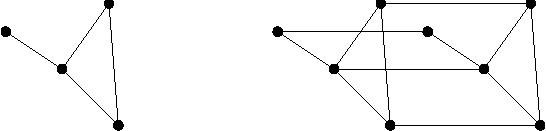
\includegraphics{double}
\end{center}
%
Some edges in the graph on the right are dashed to clarify its
structure.

\bparts

\ppart Draw the double of the graph shown below.

\vspace{0.2in}

\noindent 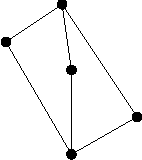
\includegraphics{youdouble}

\vspace{0.2in}

\solution{

\vspace{0.4in}
\noindent 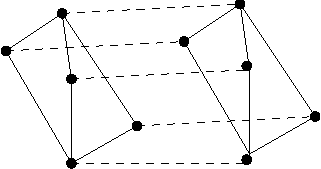
\includegraphics{youdoubleSol}

}
\newpage

\ppart Suppose that $G_1$ is a bipartite graph, $G_2$ is the double of
$G_1$, $G_3$ is the double of $G_2$, and so forth.  Use induction on
$n$ to prove that $G_n$ is bipartite for all $n \geq 1$.

\solution{We use induction.  Let $P(n)$ be the proposition that $G_n$
is bipartite.

\noindent \textit{Base case:} $P(1)$ is true because $G_1$ is
bipartite by assumption.

\noindent \textit{Inductive step:} For $n \geq 1$, we assume $P(n)$ in
order to prove $P(n+1)$.  The graph $G_{n+1}$ consists of two
subgraphs isomorphic to $G_n$ with edges joining corresponding
vertices.  Remove these extra edges.  By the assumption $P(n)$, we can
color each vertex of one subgraph black or white so that adjacent
vertices get different colors.  If we color the corresponding vertices
in the other subgraph oppositely, then adjacent vertices get different
colors within that subgraph as well.  And now if we add back the extra
edges, each of these joins a white vertex and a black vertex.
Therefore, $G_{n+1}$ is bipartite.

The theorem follows from the principle of induction.}

\eparts

\end{problem}

%%%%%%%%%%%%%%%%%%%%%%%%%%%%%%%%%%%%%%%%%%%%%%%%%%%%%%%%%%%%%%%%%%%%%%%%%%%%%%%

\newpage
\begin{problem}[12 points]  \textit{Finalphobia} is a rare disease in which
the victim has the delusion that he or she is being subjected to an
intense mathematical examination.
%
\begin{itemize}
\item A person selected uniformly at random has finalphobia with probability
$1/100$.
\item A person with finalphobia has shaky hands with probability $9/10$.
\item A person without finalphobia has shaky hands with probability $1/20$.
\end{itemize}
%
What is the probablility that a person selected uniformly at random
has finalphobia, given that he or she has shaky hands?

\solution{
Let $F$ be the event that the randomly-selected person has
finalphobia, and let $S$ be the event that he or she has shaky hands.
A tree diagram is worked out below:
%
\begin{center}
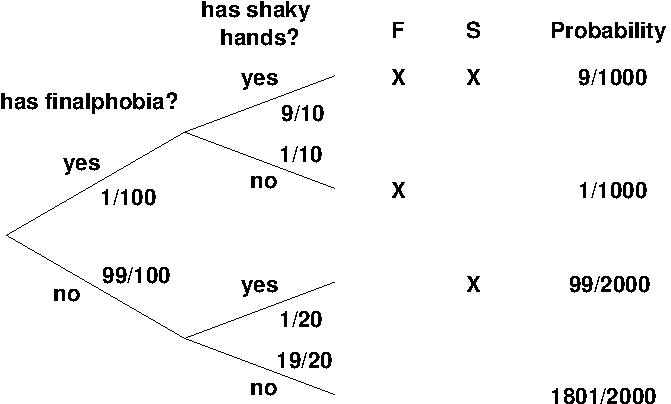
\includegraphics{finalphobia}
\end{center}
%
The probability that a person has finalphobia, given that he or she
has shaky hands is:
%
\begin{align*}
\pr{F \mid S}
    & = \frac{\pr{F \cap S}}{\pr{S}} \\
    & = \frac{9/1000}{9/1000 + 99/2000} \\
    & = \frac{18}{18+99} \\
    & = \frac{18}{117}
\end{align*}
}

\end{problem}

%%%%%%%%%%%%%%%%%%%%%%%%%%%%%%%%%%%%%%%%%%%%%%%%%%%%%%%%%%%%%%%%%%%%%%%%%%%%%%%

\newpage

\begin{problem}[12 points]
Suppose that you roll five 6-sided dice that are fair and mutually
independent.  For the problems below, answers alone are sufficient,
but we can award partial credit only if you show your work.  Also, you
do not need to simplify your answers; you may leave factorials,
binomial coefficients, and arithmetic expressions unevaluated.

\bparts

\ppart What is the probability that all five dice show different
values?

Example: $(1, 2, 3, 4, 5)$ is a roll of this type, but $(1, 1, 2, 3,
4)$ is not.

\solution[\vspace{1.75in}]{The probability space is the uniform
distribution on the $6^5$ possible numbers rolled on the five
(distinguishable) dice.  So the probability that all dice are different is
the number of outcomes in which the dice have distinct values divided by $6^5$.
There are $\paren{6}_5 = 6 \cdot 5 \cdot 4 \cdot 3 \cdot 2$ such outcomes so
\[
\pr{\text{all rolls distinct}}= \frac{6 \cdot 5 \cdot 4 \cdot 3 \cdot
2}{6^5} = \frac{5!}{6^4}
\]

An alternative approach uses the observation that the conditional
probability that the $i+1$st die value differs from the preceding rolls,
given that the first $i$ values differ, is $(6-i)/6$ for $1 \leq i \leq
4$, and the probability that all five values are different is the product
of these conditional probabilities, namely
\[
\pr{\text{all rolls distinct}} = \frac56 \cdot \frac46 \cdot\frac36 \cdot\frac26 = \frac{5!}{6^4}
\]

}

\ppart What is the probability that two dice show the same value and
the remaining three dice all show different values?

Example: $(6, 1, 6, 2, 3)$ is a roll of this type, but $(1, 1, 2, 2,
3)$ and $(4, 4, 4, 5, 6)$ are not.

\solution[\vspace{1.75in}]{
There are $\binom{5}{2}$ possible pairs of rolls that might have the same value
and 6 possibilities for what this value is.  There $5 \cdot 4 \cdot 3$
possible distinct values for the remaining three rolls.  So
\[
\pr{\text{exactly two values the same}} = \frac{\dbinom{5}{2} \cdot 6
\cdot 5 \cdot 4 \cdot 3}{6^5} = \frac{100}{6^3}
\]

An alternative way to count is: there are $\binom{6}{4}$ sets of four
values among the five dice, 4 choices for which of these values is
repeated, and by the Bookkeeper rule, $\binom{5}{2,1,1,1}= 5!/2$
permutations of a sequence consisting of five values, one of which appears
twice. So,
\[
\pr{\text{exactly two values the same}} = \frac{\dbinom{6}{4} \cdot 4
\cdot 5!/2}{6^5} = \frac{100}{6^3}
\]

}

\ppart What is the probability that two dice show one value, two
different dice show a second value, and the remaining die shows a
third value?

Example: $(6, 1, 2, 1, 2)$ is a roll of this type, but $(4, 4, 4, 4,
5)$ and $(5, 5, 5, 6, 6)$ are not.

\solution{There are $\binom{6}{2}$ sets of two values that might be
duplicated.  There are $\binom{5}{2}$ rolls where larger duplicated value
may come up and $\binom{3}{2}$ remaining rolls where the smaller
duplicated value may come up.  There is only 1 remaining roll where the
nonduplicated value may then come up, and 4 remaining values it could
take.  So,
\[
\pr{\text{exactly two pairs of same values}} =
\frac{\dbinom{6}{2} \cdot \dbinom52 \cdot \dbinom32 \cdot 4}{6^5} = \frac{50}{6^3}
\]

Alternatively, there are $\binom{6}{3}$ sets of three values among the
five dice, 3 choices for which of these values is not repeated, and by the
Bookkeeper rule, $\binom{5}{2,2,1}$ permutations of a sequence consisting
of five values, two of which appear twice. So,
\[
\pr{\text{exactly two pairs of same values}} = \frac{\dbinom{6}{3} \cdot 3
\cdot \dbinom{5}{2,2,1}}{6^5} = \frac{50}{6^3}
\]
}

\eparts

\end{problem}

%%%%%%%%%%%%%%%%%%%%%%%%%%%%%%%%%%%%%%%%%%%%%%%%%%%%%%%%%%%%%%%%%%%%%%%%%%%%%%%

\newpage

\begin{problem}[12 points]
An electronic toy displays a $4 \times 4$ grid of colored squares.  At
all times, four are red, four are green, four are blue, and four are
yellow.  For example, here is one possible configuration:
%
\begin{center}
\begin{picture}(140,130)(-30,-40)
% \put(-30,-40){\dashbox(140,130){}} % bounding box
\put(40,25){\oval(140,130)}
\multiput(0,0)(20,0){5}{\line(0,1){80}}
\multiput(0,0)(0,20){5}{\line(1,0){80}}
\multiput(0,-20)(20,0){5}{\circle{16}}
\put(0,-20){\makebox(0,0){1}}
\put(20,-20){\makebox(0,0){2}}
\put(40,-20){\makebox(0,0){3}}
\put(60,-20){\makebox(0,0){4}}
\put(80,-20){\makebox(0,0){5}}
{\Large
\put(10,10){\makebox(0,0){B}}
\put(10,30){\makebox(0,0){B}}
\put(10,50){\makebox(0,0){Y}}
\put(10,70){\makebox(0,0){R}}
\put(30,10){\makebox(0,0){G}}
\put(30,30){\makebox(0,0){R}}
\put(30,50){\makebox(0,0){B}}
\put(30,70){\makebox(0,0){B}}
\put(50,10){\makebox(0,0){Y}}
\put(50,30){\makebox(0,0){R}}
\put(50,50){\makebox(0,0){G}}
\put(50,70){\makebox(0,0){Y}}
\put(70,10){\makebox(0,0){Y}}
\put(70,30){\makebox(0,0){G}}
\put(70,50){\makebox(0,0){G}}
\put(70,70){\makebox(0,0){R}}
}
\end{picture}
\end{center}
%
For parts (a) and (b) below, you need not simplify your answers.

\bparts

\ppart How many such configurations are possible?

\solution[\vspace{2in}]{This is equal to the number of sequences
containing 4 R's, 4 G's, 4 B's, and 4 Y's, which is:
%
\[
\frac{16!}{(4!)^4}
\]
}

\ppart Below the display, there are five buttons numbered 1, 2, 3, 4,
and 5.  The player may press a sequence of buttons; however, the same
button can not be pressed twice in a row.  How many different
sequences of $n$ button-presses are possible?

\solution[\newpage]{There are 5 choices for the first button
press and 4 for each subsequence press.  Therefore, the number of
different sequences of $n$ button presses is $5 \cdot 4^{n-1}$.}

\ppart Each button press scrambles the colored squares in a
complicated, but nonrandom way.  Prove that there exist two
\textit{different} sequences of 32 button presses that both produce
the \textit{same} configuration, if the puzzle is initially in the
state shown above.  (Hint:  $4^{32} = 16^{16} > 16!$)

\solution{We use the Pigeonhole Principle.  Let $A$ be the set of all
sequences of 32 button presses, let $B$ be the set of all
configurations, and let $f : A \to B$ map each sequence of button
presses to the configuration that results.  Now:
%
\[
\size{A} > 4^{32} > 16! > \size{B}
\]
%
Thus, by the Pigeonhole Principle, $f$ is not injective; that is,
there exist distinct elements $a_1, a_2 \in A$ such taht $f(a_1) =
f(a_2)$.  In other words, there are two different sequences of button
presses that produce the same configuration}.

\eparts

\end{problem}

%%%%%%%%%%%%%%%%%%%%%%%%%%%%%%%%%%%%%%%%%%%%%%%%%%%%%%%%%%%%%%%%%%%%%%%%%%%%%%%

\iffalse
\newpage

\begin{problem}[9 points]
There are three coins:
%
\begin{itemize}
\item A nickel, which comes up heads with probability $1/4$.
\item A dime, which comes up heads with probability $1/3$.
\item A quarter, which comes up heads with probability $1/2$.
\end{itemize}
%
I select a coin uniformly at random and flip it.  If the result is
heads, what is the probability that I picked the nickel?
\end{problem}

\solution{
A tree diagram is worked out below.
%
\begin{center}
\includegraphics{finalcoins}
\end{center}
%
From the tree diagram, we have:
%
\begin{align*}
\pr{\text{nickel} \mid \text{heads}}
    & = \frac{\pr{\text{nickel} \cap \text{heads}}}
             {\pr{\text{heads}}} \\
    & = \frac{1/12}{1/12 + 1/9 + 1/6} \\
    & = \frac{3}{13}
\end{align*}
}
\fi

%%%%%%%%%%%%%%%%%%%%%%%%%%%%%%%%%%%%%%%%%%%%%%%%%%%%%%%%%%%%%%%%%%%%%%%%%%%%%%%

\newpage

\begin{problem}[12 points]
MIT students sometimes delay laundry for a few days.  Assume all
random values described below are mutually independent.

\bparts

\ppart A \term{busy} student must complete 3 problem sets before doing
laundry.  Each problem set requires 1 day with probability $2/3$ and 2
days with probability $1/3$.  Let $B$ be the number of days a busy
student delays laundry.  What is $\ex{B}$?

Example: If the first problem set requires 1 day and the second and
third problem sets each require 2 days, then the student delays for $B
= 5$ days.

\solution[\vspace{2.5in}]{ The expected time to complete a problem
set is:
%
\[
1 \cdot \frac{2}{3} + 2 \cdot \frac{1}{3} = \frac{4}{3}
\]
%
Therefore, the expected time to complete all three problem sets is:
%
\begin{align*}
\ex{B}
    & = \ex{\text{pset1}} + \ex{\text{pset2}} + \ex{\text{pset3}} \\
    & = \frac{4}{3} + \frac{4}{3} + \frac{4}{3} \\
    & = 4
\end{align*}
}

\ppart A \term{relaxed} student rolls a fair, 6-sided die in the
morning.  If he rolls a 1, then he does his laundry immediately (with
zero days of delay).  Otherwise, he delays for one day and repeats the
experiment the following morning.  Let $R$ be the number of days a
relaxed student delays laundry.  What is $\ex{R}$?

Example: If the student rolls a 2 the first morning, a 5 the second
morning, and a 1 the third morning, then he delays for $R = 2$ days.

\solution[\newpage]{If we regard doing laundry as a failure, then the
mean time to failure is $1 / (1/6) = 6$.  However, this counts the day
laundry is done, so the number of days delay is $6 - 1 = 5$.
Alternatively, we could derive the answer as follows:
%
\begin{align*}
\ex{R}
    & = \sum_{k=0}^{\infty} \pr{R > k} \\
    & = \frac{5}{6} + \paren{\frac{5}{6}}^2 + \paren{\frac{5}{6}}^3 + \ldots \\
    & = \frac{5}{6} \cdot
            \paren{1 + \frac{5}{6} + \paren{\frac{5}{6}}^2 + \ldots} \\
    & = \frac{5}{6} \cdot \frac{1}{1 - 5/6} \\
    & = 5
\end{align*}
}

\ppart Before doing laundry, an \term{unlucky} student must recover
from illness for a number of days equal to the product of the numbers
rolled on two fair, 6-sided dice.  Let $U$ be the expected number of
days an unlucky student delays laundry.  What is $\ex{U}$?

Example: If the rolls are 5 and 3, then the student delays for $U =
15$ days.

\solution[\vspace{3in}]{Let $D_1$ and $D_2$ be the two die rolls.
Recall that a die roll has expectation $7/2$.  Thus:
%
\begin{align*}
\ex{U}
    & = \ex{D_1 \cdot D_2} \\
    & = \ex{D_1} \cdot \ex{D_2} \\
    & = \frac{7}{2} \cdot \frac{7}{2} \\
    & = \frac{49}{4}
\end{align*}
}

\ppart A student is \term{busy} with probability $1/2$, \term{relaxed}
with probability $1/3$, and \term{unlucky} with probability $1/6$.
Let $D$ be the number of days the student delays laundry.  What is
$\ex{D}$?  \textit{Leave your answer in terms of $\ex{B}$, $\ex{R}$,
and $\ex{U}$.}

\solution{
\[
\ex{D} = \frac{1}{2} \ex{B} + \frac{1}{3} \ex{R} + \frac{1}{6} \ex{U}
\]
}

\eparts

\end{problem}

%%%%%%%%%%%%%%%%%%%%%%%%%%%%%%%%%%%%%%%%%%%%%%%%%%%%%%%%%%%%%%%%%%%%%%%%%%%%%%%

\newpage

\begin{problem}[12 points]
I have twelve cards:
%
\[
\fbox{1}\ \fbox{1}\quad \fbox{2}\ \fbox{2}\quad \fbox{3}\ \fbox{3}\quad
\fbox{4}\ \fbox{4}\quad \fbox{5}\ \fbox{5}\quad \fbox{6}\ \fbox{6}
\]
%
I shuffle them and deal them in a row.  For example, I might get:
%
\[
\fbox{1}\ \fbox{2}\ \fbox{3}\ \fbox{3}\ \fbox{4}\ \fbox{6}\ 
\fbox{1}\ \fbox{4}\ \fbox{5}\ \fbox{5}\ \fbox{2}\ \fbox{6}
\]
%
What is the expected number of adjacent pairs with the same value?  In
the example, there are two adjacent pairs with the same value, the 3's
and the 5's.

We can award partial credit only if you show your work.
\end{problem}

\solution{Consider an adjacent pair.  The left card matches only one
of the other 11 cards, which is equally likely to be in any of the 11
other positions.  Therefore, the probability that an adjacent pair
matches is $1/11$.  Since there are 11 adjacent pairs, the expected
number of matches is $11 \cdot 1/11 = 1$ by linearity of expectation.}

%%%%%%%%%%%%%%%%%%%%%%%%%%%%%%%%%%%%%%%%%%%%%%%%%%%%%%%%%%%%%%%%%%%%%%%%%%%%%%%

\newpage

\begin{problem}[12 points]
Each time a baseball player bats, he hits the ball with some
probability.  The table below gives the hit probability and number of
chances to bat next season for five players.
%
\begin{center}
\begin{tabular}{ccc}
player & prob. of hit & \# chances to bat \\[0.5ex]
Player A & $1/3$ & 300 \\
Player B & $1/4$ & 200 \\
Player C & $1/4$ & 400 \\
Player D & $1/5$ & 250 \\
Player E & $2/5$ & 500
\end{tabular}
\end{center}
\bparts

\ppart Let $X$ be the total number times these five players hit the
ball next season.  What is $\ex{X}$?

\solution[\vspace{2.5in}]{The expected number of events that happen is
equal to the sum of the event probabilities.  So we have:
%
\begin{align*}
\ex{X}
    & = 300 \cdot \frac{1}{3} + 200 \cdot \frac{1}{4}
      + 400 \cdot \frac{1}{4} + 250 \cdot \frac{1}{5}
      + 500 \cdot \frac{2}{5} \\
   & = 100 + 50 + 100 + 50 + 200 \\
   & = 500
\end{align*}
}

\ppart Give a nontrivial upper bound on $\pr{X \geq 1500}$ and justify
your answer.  \textit{Do not} assume that hits happen mutually
independently.

\solution[\newpage]{We use the Markov Inequality:
%
\[
\pr{X \geq c} \leq \frac{\ex{X}}{c}
\]
%
This gives:
\begin{align*}
\pr{X \geq 1500}
    & \leq \frac{\ex{X}}{1500} \\
    & = \frac{1}{3}
\end{align*}
}

\ppart Using a Chernoff inequality, give a nontrivial upper bound on
$\pr{X \leq 400}$.  For this part, you \textit{may} assume that all
hits happen mutually independently.

\solution{
We use the Chernoff Inequality:
%
\[
\pr{X \leq (1 - \delta) \ex{X}} \leq e^{\textstyle - \delta^2 \ex{X} / 2}
\]
%
This gives:
%
\begin{align*}
\pr{X \leq 400}
    & = \pr{X \leq (1 - 1/5) \ex{X}} \\
    & \leq e^{-(1/5)^2 500 / 2} \\
    & = e^{-10}
\end{align*}
}

\eparts

\end{problem}

%%%%%%%%%%%%%%%%%%%%%%%%%%%%%%%%%%%%%%%%%%%%%%%%%%%%%%%%%%%%%%%%%%%%%%%%%%%%%%%
%\includepdf[angle=-90,offset=40 -90,landscape]{FinalHist.pdf}


\end{document}
